\documentclass[10pt,tgadventor, onlymath]{beamer}

\usepackage{graphicx,amsmath,amssymb,tikz,psfrag,neuralnetwork}

%\input defs.tex
\graphicspath{ {./figures/} }

%% formatting

\mode<presentation>
{
\usetheme{default}
\usetheme{Berlin}

\usecolortheme{seahorse}
}
\setbeamertemplate{navigation symbols}{}
\usecolortheme[rgb={0.03,0.28,0.59}]{structure}
\setbeamertemplate{itemize subitem}{--}
\setbeamertemplate{frametitle} {
	\begin{center}
	  {\large\bf \insertframetitle}
	\end{center}
}

\newcommand\footlineon{
  \setbeamertemplate{footline} {
    \begin{beamercolorbox}[ht=2.5ex,dp=1.125ex,leftskip=.8cm,rightskip=.6cm]{structure}
      \footnotesize \insertsection
      \hfill
      {\insertframenumber}
    \end{beamercolorbox}
    \vskip 0.45cm
  }
}
\footlineon

\AtBeginSection[] 
{ 
	\begin{frame}<beamer> 
		\frametitle{Outline} 
		\tableofcontents[currentsection,currentsubsection] 
	\end{frame} 
} 


\tikzstyle{state}=[shape=circle,draw=blue!30,fill=blue!10]
\tikzstyle{observation}=[shape=rectangle,draw=orange!30,fill=orange!10]
\tikzstyle{lightedge}=[<-, dashed]
\tikzstyle{mainstate}=[state, thick]
\tikzstyle{mainedge}=[<-, thick]
\tikzstyle{block} = [draw,rectangle,thick,minimum height=2em,minimum width=2em]
\tikzstyle{sum} = [draw,circle,inner sep=0mm,minimum size=2mm]
\tikzstyle{connector} = [->,thick]
\tikzstyle{line} = [thick]
\tikzstyle{branch} = [circle,inner sep=0pt,minimum size=1mm,fill=black,draw=black]
\tikzstyle{guide} = []
\tikzstyle{snakeline} = [connector, decorate, decoration={pre length=0.2cm,
                         post length=0.2cm, snake, amplitude=.4mm,
                         segment length=2mm},thick, magenta, ->]



%% begin presentation

\title{\large \bfseries Asymptotic Capacity of Systems with Intelligent Reflective Surface}

\author{Peter Hartig\\[3ex]}

\date{\today}

\begin{document}

\frame{
\thispagestyle{empty}
\titlepage
}

\section{Background}
\subsubsection{Devices}
\begin{frame}
\frametitle{Relaying}

	\begin{itemize}
		\item 			
			Relays vs. base-stations
		\item 
			Different modes of operation (Decode and forward, amplify and forward ...)
		\item 
			Extending wireless coverage is relevant to high frequencies used in 5G +
	\end{itemize}
\end{frame}

\begin{frame}
\frametitle{Intelligent Reflective surface: Under the Hood}
\begin{columns}
\begin{column}{0.5\linewidth}
	Mode 1
	\begin{figure}
%			\centering
		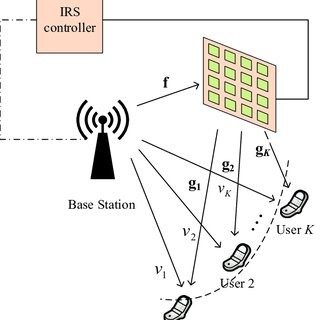
\includegraphics[scale=1]{irs}
	\end{figure}\end{column}
\begin{column}{0.5\linewidth}
	Information Assumptions

\end{column}
\end{columns}
\end{frame}


\begin{frame}
\frametitle{IRS: Modes of Operation}
\begin{columns}
\begin{column}{0.5\linewidth}
	Mode 1
	\begin{figure}
%			\centering
		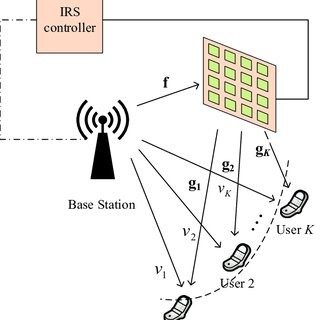
\includegraphics[scale=1]{irs}
	\end{figure}\end{column}
\begin{column}{0.5\linewidth}
	Mode 2 (The one we will use)

\end{column}
\end{columns}
\end{frame}

\begin{frame}
\frametitle{Resulting Impact on Signal}
\centering
\begin{equation}
\mathbf{y} = \mathbf{H}_2\boldsymbol{\Theta}\mathbf{H}_1\mathbf{F}\mathbf{x}
\end{equation}
\end{frame}


\begin{frame}
\frametitle{Relays vs. IRS}
\begin{itemize}
\item difference
\end{itemize}
\end{frame}


\subsubsection{Relevant MIMO Information Theory}
\begin{frame}
\frametitle{Multiple Scattering}
System Model
\begin{equation}
t
\end{equation}
Asymptotic analysis

\end{frame}

\begin{frame}
\frametitle{Concatenated Scattering}
\begin{equation}
t
\end{equation}
\end{frame}

\section{Goals}
\begin{frame}
\frametitle{Project Goals}
\begin{enumerate}
\item
	Find capacity of asymptotic IRS systems with random IRS phases (equivalent to scattering)
\item 
	Find capacity with phases optimized according to what objective function
\item
	Extend random phase results to secrecy capacity
\item
	Investigate optimizing phases for maximizing secrecy capacity
\item 
	Confirm findings with numerical results
\end{enumerate}
\end{frame}

\section{Current Status}



\begin{frame}
\frametitle{Next Steps}

\end{frame}


\section{Conclusion}

\begin{frame}
  \centering \Large
  \emph{Thank You.}
  \\
	\bigskip
    \centering \Large
  \emph{Questions or Comments?}

\end{frame}





\end{document}
